% Figure 11.1 redrawn from PDF page 333. Figures 11.2 and 11.3 retain
% the original anatomical illustrations (PDF pages 362--363); only labels
% are covered by Chinese TeX text, leaving patient figures and colors intact.
\providecommand{\chElevenTrial}{\begin{tikzpicture}[font=\footnotesize,>=Stealth]
\draw[dashed,dcrred] (0,0) ellipse (2.6 and 2.8);\node[text=dcrred]at(0,3.1){可接触人群};
\node[align=center]at(0,2.1){符合选择标准的参与者};
\node[draw=dcrred,text width=36mm,minimum height=31mm,align=center,text=dcrpurple](b)at(0,0){测量基线变量\\[10pt]保存标本（可选）};
\node[circle,draw,minimum size=10mm](r)at(3.6,0){R};\draw[->](b)--(r);
\node[draw=dcrteal,text width=47mm,align=left](a)at(7.8,1.6){\textcolor{dcrblue}{实施设盲干预}\\测量依从\\\textcolor{dcrgold}{结局发生时测量}};
\node[draw=dcrteal,text width=47mm,align=left](c)at(7.8,-1.6){\textcolor{dcrblue}{实施设盲对照}\\测量依从\\\textcolor{dcrgold}{结局发生时测量}};
\draw[->,dcrteal](r)to[bend left=25](a);\draw[->,dcrteal](r)to[bend right=25](c);
\node[draw=dcrgold,text=dcrgold,align=center](e)at(11.5,0){也可在\\随访结束时\\测量结局};
\draw[->,dcrteal](a)--(e);\draw[->,dcrteal](c)--(e);
\foreach \yy in {1.6,-1.6}{\draw[->,dcrteal](7,\yy-.6)to[bend left=30](7.4,\yy-1.1);\draw[->,dcrteal](8.4,\yy-.6)to[bend left=30](8.8,\yy-1.1);\node[text=dcrteal]at(7.9,\yy-1.35){失访};}
\end{tikzpicture}}
\providecommand{\chElevenHip}{\begin{tikzpicture}[x=.018cm,y=-.018cm]
\node[anchor=north west,inner sep=0]at(0,0){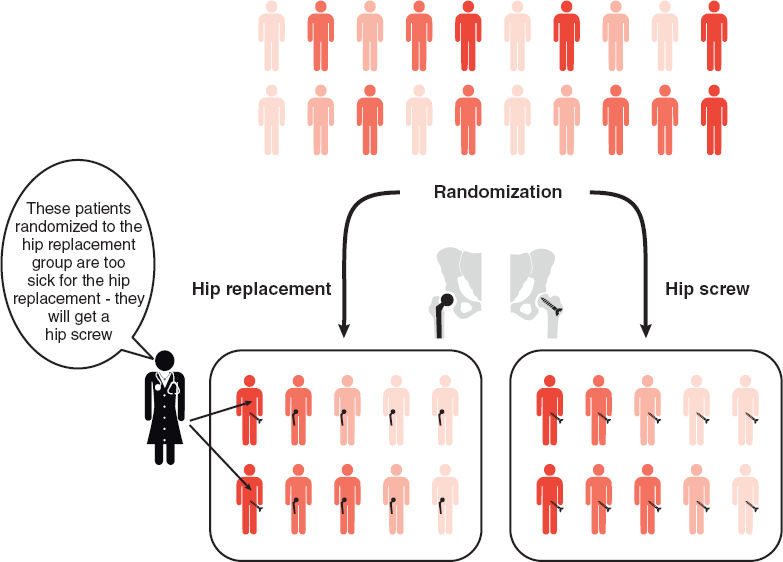
\includegraphics[width=14.094cm]{assets/ch11_figure02_original.png}};
\fill[white](403,174)rectangle(595,208);\node[font=\small]at(500,191){随机分组};
\fill[white](186,271)rectangle(334,305);\node[font=\small]at(260,289){髋关节置换};
\fill[white](653,271)rectangle(778,305);\node[font=\small]at(715,289){髋螺钉固定};
\fill[white](78,264)ellipse(73 and 100);
\node[text width=1.8cm,align=center,font=\scriptsize,fill=white]at(80,273){这些患者虽随机分入置换组，但病情太重，不适合置换，将改用螺钉固定。};
\end{tikzpicture}}
\providecommand{\chElevenAnalysis}{\begin{tikzpicture}[x=.018cm,y=-.018cm]
\node[anchor=north west,inner sep=0]at(0,0){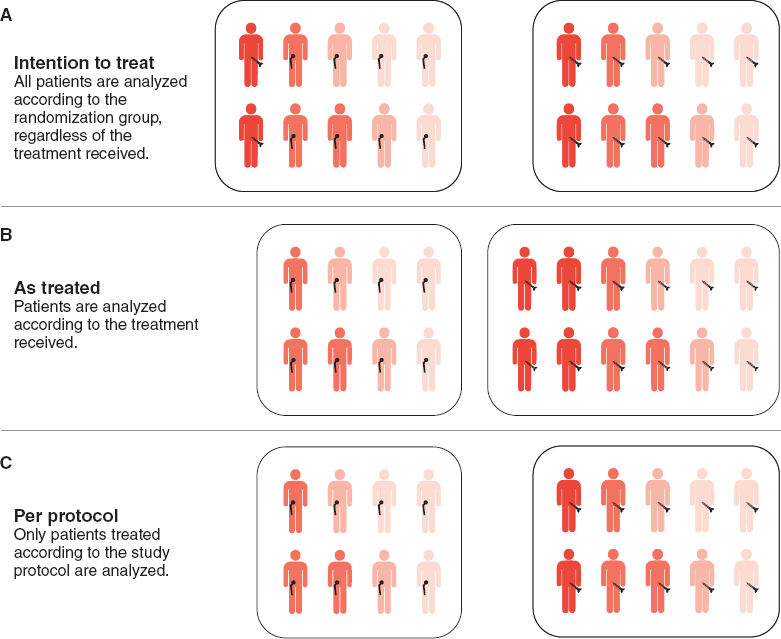
\includegraphics[width=14.058cm]{assets/ch11_figure03_original.png}};
\fill[white](5,35)rectangle(210,181);\node[anchor=west,text width=3.3cm,align=left,font=\small]at(14,103){\textbf{意向治疗分析}\\全部患者按随机分组分析，不管实际治疗。};
\fill[white](5,266)rectangle(210,390);\node[anchor=west,text width=3.3cm,align=left,font=\small]at(14,326){\textbf{按实际治疗分析}\\按实际接受的治疗分析。};
\fill[white](5,486)rectangle(210,609);\node[anchor=west,text width=3.3cm,align=left,font=\small]at(14,547){\textbf{符合方案分析}\\仅分析按研究方案治疗的患者。};
\end{tikzpicture}}
